% Figure -- headline FID + designability convergence. \input{} from Ch6.
\begin{figure}[tbp]
\centering
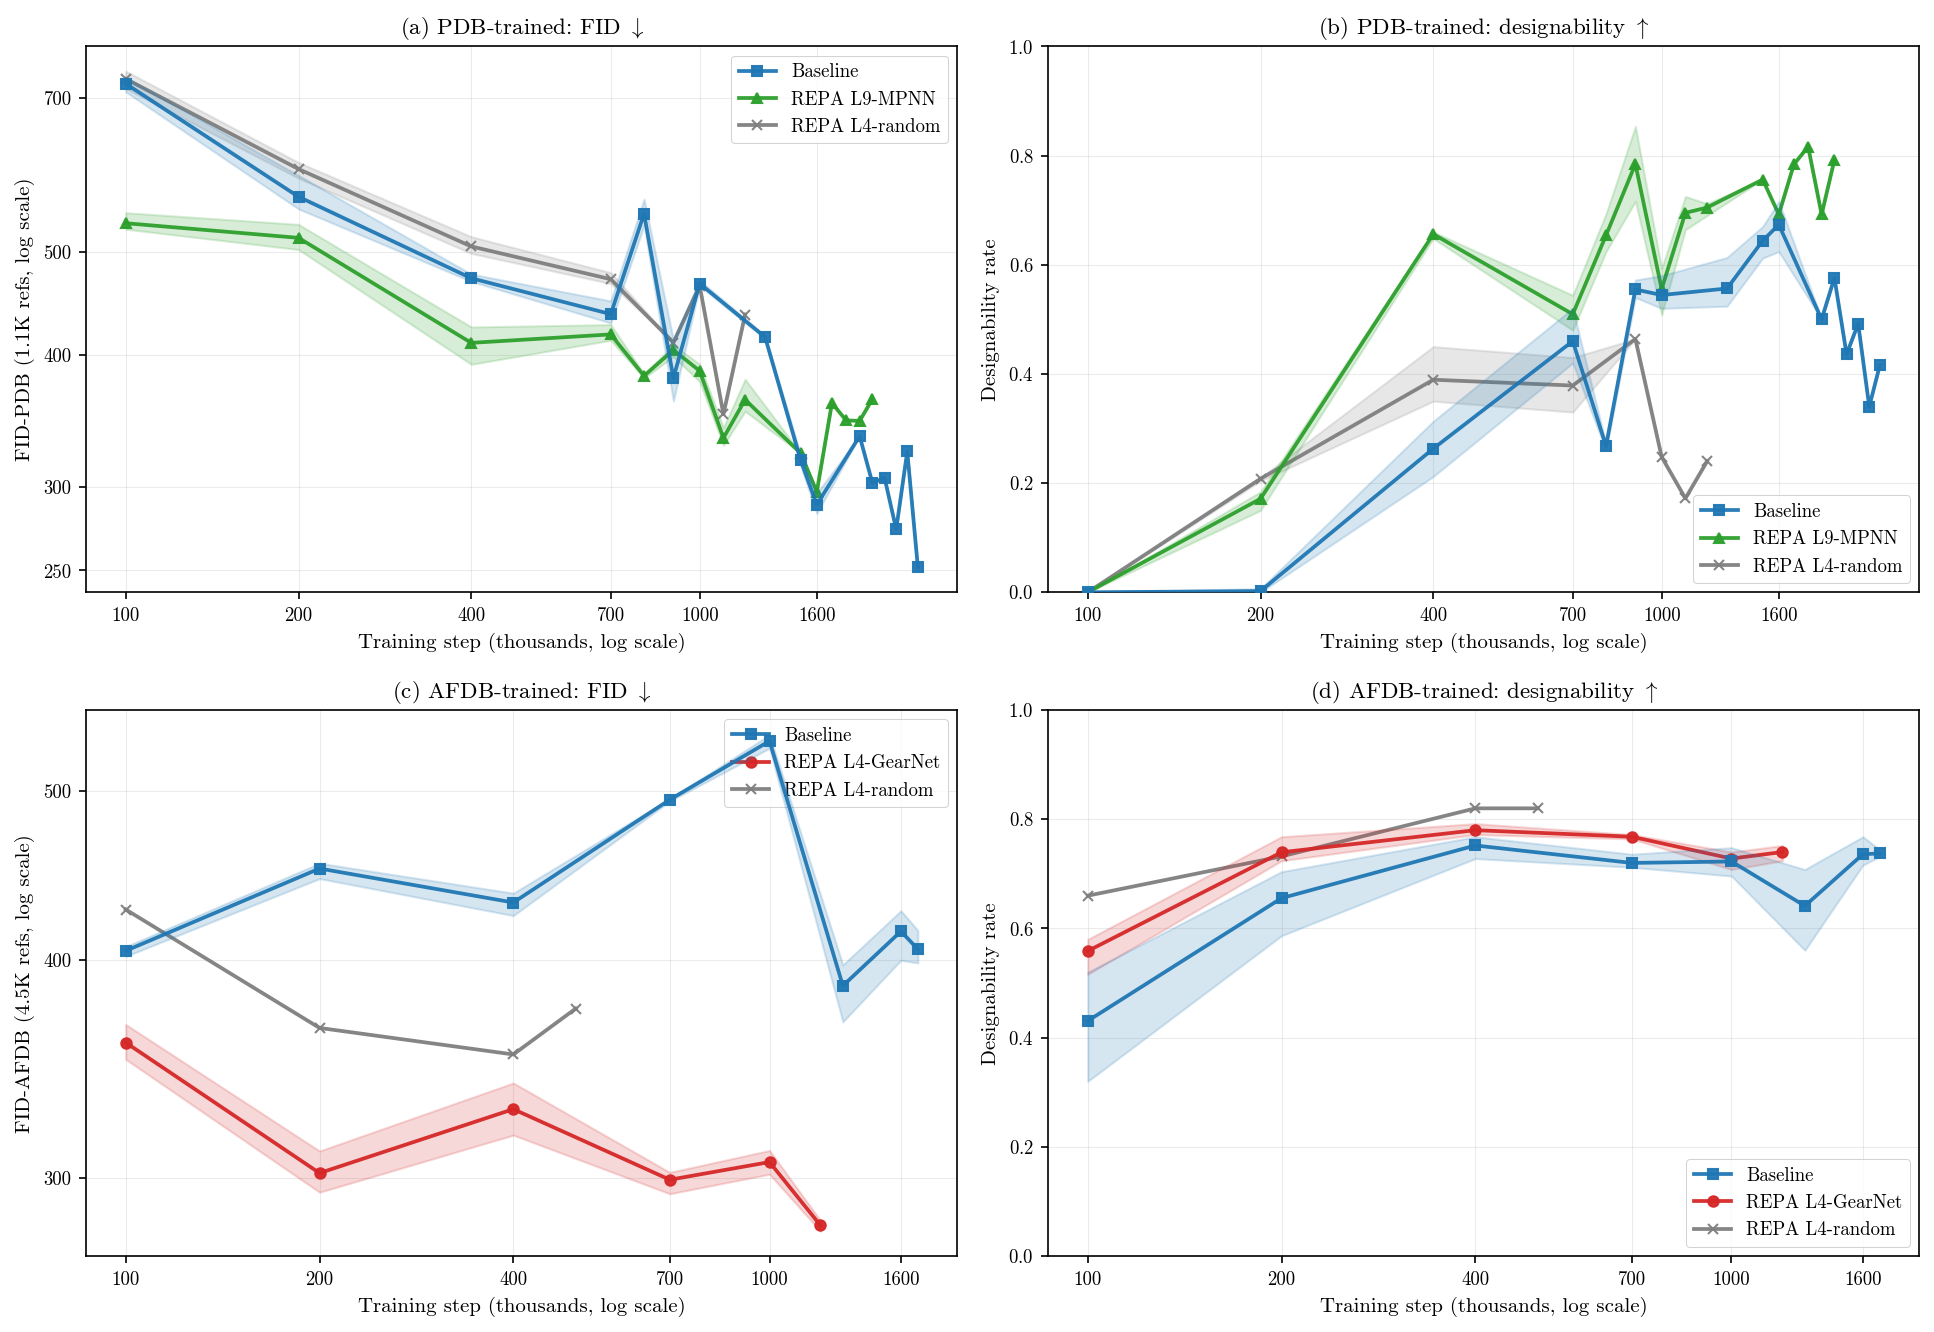
\includegraphics[width=\textwidth]{figures/fig01_fid_des_convergence.png}
\caption{\textbf{REPA accelerates both FID and designability, in both PDB (experimental) and AFDB (synthetic) data regimes.} The random-encoder control (grey) helps distinguish gains induced by regularisation alone from those induced mechanistically by an encoder's learned structure. While PDB retains a persistent designability gap, its baseline appears to catch up on FID after $\approx$1M steps; we examine this in \S\ref{sec:proteina-convergence}. ($n{\le}256$ models, 3 seeds; shaded bands show min/max.)}
\label{fig:proteina-fid}
\end{figure}
